\documentclass[%
    %draft,
    %submission,
    %compressed,
    final,
    %
    %technote,
    %internal,
    %submitted,
    %inpress,
    reprint,
    %
    %titlepage,
    notitlepage,
    %anonymous,
    narroweqnarray,
    inline,
    twoside,
    invited
    ]{ieee}

\usepackage[utf8]{inputenc}
\usepackage[spanish]{babel}
\usepackage{graphicx}
\usepackage{verbatim}
\usepackage{moreverb}
\usepackage{amsmath}
\usepackage{amsfonts}
\usepackage{amssymb}
\usepackage{fancybox}
\usepackage{float}
\usepackage{fancyvrb}
\usepackage{subfigure}

\newcommand{\latexiie}{\LaTeX2{\Large$_\varepsilon$}}

%\usepackage{ieeetsp}    % if you want the "trans. sig. pro." style
%\usepackage{ieeetc}    % if you want the "trans. comp." style
%\usepackage{ieeeimtc}    % if you want the IMTC conference style

% Use the `endfloat' package to move figures and tables to the end
% of the paper. Useful for `submission' mode.
%\usepackage {endfloat}

% Use the `times' package to use Helvetica and Times-Roman fonts
% instead of the standard Computer Modern fonts. Useful for the 
% IEEE Computer Society transactions.
%\usepackage{times}
% (Note: If you have the commercial package `mathtime,' (from 
% y&y (http://www.yandy.com), it is much better, but the `times' 
% package works too). So, if you have it...
%\usepackage {mathtime}

% for any plug-in code... insert it here. For example, the CDC style...
%\usepackage{ieeecdc}

\begin{document}

%----------------------------------------------------------------------
% Title Information, Abstract and Keywords
%----------------------------------------------------------------------
\title[Métodos de búsqueda no informados e informados]{%
       Métodos de búsqueda no informados e informados}

% format author this way for journal articles.
% MAKE SURE THERE ARE NO SPACES BEFORE A \member OR \authorinfo
% COMMAND (this also means `don't break the line before these
% commands).
\author[Castiglione, Karpovsky, Sturla]{Gonzalo V. Castiglione, Alan E. Karpovsky, Martín Sturla\\\textit{Estudiantes 
       Instituto Tecnológico de Buenos Aires (ITBA)}\\
\\\textbf{20 de Marzo de 2012}
}



\journal{Cátedra\ \ Sist.\ de\ Inteligencia\ Artificial,\ ITBA\ }
\titletext{-\ 20, MARZO\ 2012}
\ieeecopyright{\copyright\ 2012 ITBA}
\lognumber{}
\pubitemident{}
\loginfo{20 de Marzo, 2012.}
\firstpage{1}

\confplacedate{Buenos Aires, Argentina, 20 de Marzo, 2012}

\maketitle               

\begin{abstract} 
El presente informe busca analizar y comparar distintas estrategias de búsqueda sobre un problema en particular (Skyscraper puzzle) haciendo uso de un motor de inferencias, como así también evaluar las mejoras obtenidas mediante la aplicación de heurísticas.
\end{abstract}

\begin{keywords}
DFS, BFS, General Problem Solver, depth-first, breadth-first, search strategy, iterative DFS, A Star
\end{keywords}

%----------------------------------------------------------------------
% SECTION I: Introduccion%----------------------------------------------------------------------
\section{Introducción}

\PARstart El juego \textit{Edificios} también conocido como \textit{Skyscraper puzzle} es una variante del conocido \textit{Sudoku} y consiste de una grilla cuadrada con números en su borde que representan las pistas sobre cuántos edificios se visualizan en esa dirección. El tablero, visto desde arriba, representa un espacio cubierto de edificios. Cada casillero debe ser completado con un dígito que va entre 1 y N, siendo N el tamaño de la grilla; haciendo que cada fila y cada columna contengan sólo una vez a cada dígito (como sucede en el Sudoku).

%\par En este puzzle, cada dígito puesto en la grilla podría ser visualizado como un edificio de %esa altura. Por ejemplo, si ingresamos un 5, estaríamos colocando un edificio de altura 5. Cada %uno de los numeros que están por fuera de la grilla revelan la cantidad de edificios que pueden %ser vistos al mirar la línea o columna en esa dirección. Cada edificio bloquea la visión de todo %edificio de menor altura que se encuentre detrás de él.

%----------------------------------------------------------------------
% SECTION II: Marco Teórico
%----------------------------------------------------------------------

\section{Estados del problema}

\subsection{Estado inicial}

\par El estado inicial del problema es un tablero que contiene sólo las pistas en sus bordes (no contiene ningún edificio en la grilla). 
Para que el problema tenga solución éste tablero debe ser válido; es decir que no cualquier combinación de pistas sobre la visibilidad
 de edificios en esa dirección conducirán a un problema resoluble.

\subsection{Estado final}

\par El estado final del problema es un tablero con todos los casilleros completos (lleno de edificios) que cumpla con las reglas 
del juego citadas anteriormente.

\section{Modelado del problema}

\par El tablero del juego se modeló mediante la creación de la clase Board; la misma contiene una variable privada de tipo matriz de 
enteros que representa a la grilla propiamente dicha. Si un casillero de dicha matriz  tiene un $0$, significa que  está vacío; si en cambio 
tiene un número $k \in [1,n]$ significa que hay situado un edificio con altura $k$. El tablero contiene además algunas variables necesarias para 
incrementar la performance de ciertas heurísticas explicadas adelante. Entre dichas variables se encuentra las coordenadas del último edificio puesto.\\
\par Las pistas o restricciones del tablero (números en los bordes del mismo) se modelaron con un arreglo de cuatro 
vectores de enteros (TOP, BOTTOM, LEFT, RIGHT) que simplemente contienen la restricción en esa dirección.
Cabe destacar que en los estados únicamente se guarda el tablero; guardar las restricciones sería redundante. 
Ver \textbf{Figura 1} en la sección \textbf{Anexo B}.\\



\section{Reglas}

\par Para la resolución de este problema se han pensado dos conjuntos de reglas distintos. El primero, enunciado a continuación, fue descartado por su baja performance. Seguido de este se explicará el conjunto de reglas elegido y sus beneficios.\\

\par Dado un tablero de tamaño $n\times n$ podemos describir las reglas del problema en forma general como sigue:\\

\emph{Poner un edificio de altura $x$ en la posición $(i,j)$ del tablero, con $x \in [1, n]$.}\\

\par Por lo que, que dado un tablero de $n\times n$, el total de reglas está dado por $n \times {n \times n} = n^3$ ya que por cada fila y por cada columna, se tienen $n$ edificios distintos para colocar. 
\par Ejemplos de reglas:
\begin{itemize}
\item Poner un edificio de altura 1 en la posición $(0,0)$
\item Poner un edificio de altura 4 en la posición $(3,1)$
\item $\ldots$

\end{itemize}

\par Las reglas así definidas producen un factor de ramificación de $n^3$ lo que hace que, para tableros grandes (mayores a $5\times5$) se 
tarde un tiempo muy considerable (en el orden de las horas) en encontrar la solución. Además este conjunto de rueglas tiene el problema 
de ser mayormente conmutativas. Esto crea muchos estados redundantes. 
Para subsanar este inconveniente se puede plantear el problema enunciando con un conjunto de reglas distinto, descripto a continuación:\\

\emph{Poner un edificio de tamaño $x$ en el próximo lugar disponible de izquierda a derecha y de arriba hacia abajo, con $x \in [1, n]$.}\\

\par En un tablero de $n\times n$ el conjunto de reglas quedaría definido de la siguiente forma:\\

\begin{itemize}
\item Poner un edificio de altura 1 en el próximo lugar disponible según el recorrido usado.
\item $\vdots$
\item Poner un edificio de altura $n$ en el próximo lugar disponible según el recorrido usado.
\end{itemize}

\par Esto otorga un factor de ramificación igual a $n$ siendo este muy inferior al del caso anterior. El próximo casillero a llenar está indicado por 
el recorrido. Más adelante se enumerarán los recorridos y sus respectivas propiedades, ventajas y desventajas. \\
\par Para la primer etapa se decidió implementar ambos conjuntos de reglas y los resultados fueron comparados en las tablas de la sección \textbf{Anexo A}. 
Para la segunda etapa del trabajo se decidió utilizar únicamente el segundo conjunto de reglas, utilizando distintos recorridos y comparándolos (reference needed). 

\section{Costos}

\par Debido a la naturaleza del probema, la aplciacion de todas las reglas tiene el mismo costo y éste es unitario. Es decir que la transición de un estado X a un estado Y, en nuestro caso, siempre cuesta $1$.

\section{Algoritmos de búsqueda implementados}

\par Hemos implementado seis algoritmos de búsqueda no informada diferentes. Los mismos son: DFS, BFS, IDFS, HIDFS, Greedy search y AStar \textit{(A*)}.

\section{Heurísticas}

\par Como se ha planteado el modelado del problema, tiene poco sentido hablar de una función heurística que estime el costo de un cierto nodo 
a la solución. Esto se debe a que la profundidad de la solución es sabida de antemano. Sin embargo, es válido plantear que si un nodo 
no tiene solución porque ninguna asignación de valores de las variables o casilleros aún incompletos satisface las restricciones del problema. Por lo tanto, 
se decidió asignar a la función heurística un costo unitario por cada casillero aún no asignado si el tablero aún parece tener solución, e infinito 
si no se puede alcanzar la solución. Los nodos marcados con un valor de $h$ infinito permanecerán en la frontera y nunca serán explotados a menos que 
el problema no tenga solución.
\par Se centró el estudio de los tableros sin soluciones en base a las restricciones dadas por los números fuera del tablero, numeradas a continuación.\\

\subsection{Propiedad 1}

\par Si una restricción indica el número $1$, esa fila o columna deberá comenzar con la altura maxima $(n)$. Además si la restricción opuesta es un $2$, se coloca $n-1$ al lado de este.

\subsection{Propiedad 2}

\par Dado un tablero de dimensión $n$, si una restricción indica algún número distinto de $1$ , esa fila o columna trivialmente no podrá comenzar con $(n)$.\\
\par Si se considera el caso general, si una restricción indica algún número $a$ mayor o igual que $1$ , esa fila o columna deberá tener un edificio con la altura máxima $(n)$ a, al menos, $a$ casilleros de distancia.  Si generalizamos este resultado, podemos obtener el siguiente resultado útil:\\\\
\emph{Dado una fila o columna con restricción $n$, para cada edificio de altura $k$ tenemos $dist(k) >= a + k - n - 1 $, siendo $n$ la dimensión del tablero y $a$ la restricción a validar.}\\
\par En otras palabras, el edificio de altura máxima debe estar a $n$ casilleros de distancia, el de altura $n-1$ a distancia $n-1$ o mayor, y así sucesivamente. Esto implica que los edificios deben estar ordenados de menor a mayor si se da esta situación.

\par Estas dos heurísticas previas se combinaron con las restricciones de  \textit{naturaleza Sudoku} del problema, es decir la restricción \texit{alldif} 
que existe en cada fila y columna (es decir, todos los valores deben ser distintos) para intentar maximizar el hallazgo de nodos irresolubles.\\

\subsection{Valor heurístico de un estado}

\par Si un estado no conducirá de ninguna manera a una solución, asignar el valor \textit{infinito} a ese estado. 
\par Durante el desarrollo del trabajo se analizaron distintos valores heurísticos que se le puede asignar a aquellos estados que no han sido 
identificados como irresolubles. A continuación se enumeraron las opciones:

\subsubsection{Costo simple}

\par Consiste en asignar simplemente la cantidad de casilleros aún no completados como valor de $h$. Es fácil ver que esta asignación favorece el explotado
 de nodos con mayor profundidad, lo cual dio mejores resultados que sus contrapartes. Esta función heurística es trivialmente admisible dado que:
\begin{itemize}
\item Si un estado es soluble y es considerado soluble, $h$ es exactamente la longitud del camino más corto a una solución.
\item Si un estado es irresoluble y no se lo ha identificado como tal, $h$ es trivialmente una subestimación de la longitud del camino más corto a la solucion.
\item Si un estado es irresoluble y se lo ha identificado como tal, $h$ es teóricamente la longitud del camino a la solución,  infinito, pero en la práctica 
es una subestimación debido a limitaciones del tamaño de almacenamiento.
\end{itemize}

\subsubsection{Análisis de la restrictividad de un estado}

\par Evaluar la \textit{restrictividad} de un determinado estado según la \textbf{selección de valores} ( y no la de variables, que será 
discutida más adelante). Este es un índice que se crea calculando la cantidad de posibles números que se pueden colocar 
en cada casillero aún incompleto, intentando ser normalizado según la cantidad de casilleros ya completos, dado que tableros más completos son trivialmente más 
restrictivos que tableros más vacíos. Por un lado, se investigó la penalización de tableros poco restrictivos para favorecer
 a estados con menor ramificación y sucesores. Por otro lado se investigó la penalización de tableros más restrictivos, con el pretexto de que 
mucha restrictividad implica poca probabilidad de hallar una solución, sobre todo si aún hay muchos casilleros para completar.
\par Para penalizar dichos tableros, sea cual sea el criterio, se incrementó el valor de $h$ por arriba de la cantidad de casilleros sin llenar. Esto hace 
que la heurística sea trivialmente no admisible. Sin embargo, la admisibilidad de una heurística garantiza en el algoritmo \textit{A*} la optimalidad. Dado 
que en este problema la solución tiene siempre la misma profundiad, no existe tal cosa como una solución más óptima que otra. En vista de esto se decidió 
implementar dicha heuristica y comparar los resultados.
\section{Recorridos}

\par Se han implementado tres tipos de recorridos distintos sobre el tablero, en busca de comparar la performance obtenida con cada uno de ellos.\\

\begin{itemize}
\item \textbf{Recorrido secuencial: } Se avanza de izquierda a derecha, desde arriba hacia abajo.
\item \textbf{Recorrido en espiral: } Se avanza desde el centro en forma de espiral o desde una esquina hacia al centro, de forma análoga.
\item \textbf{Recorrido MVR: } Se avanza hacia el casillero con menor cantidad de valores legales (mayor restrictividad). Nótese que se apunta 
a mayor restrictividad en cuanto a la \textbf{selección de variables o casilleros}. Cabe destacar que esto no 
entra en conflicto las heurísticas recién planteadas. Por ejemplo, se podría penalizar con heurísticas tableros muy restrictivos, y aún aplicar este 
recorrido. En esencia lo que se hace en cada paso es buscar el casillero con menor cantidad de posibles asignaciones de valores, generar un sucesor 
con cada uno de estos, pero explotar primero el que hace que el resto de los casilleros tenga la menor restrictividad posible. Esto se denomina 
\textit{ variable selection fail-first, value selection fail-last}. Para mayores referencias se puede consultar el libro de Russel y Norvig.
\end{itemize}

\section{Resultados}

\subsection{Algoritmos}

\par A través de las distintas pruebas realizadas se observó que para las búsquedas no informadas, el algoritmo con mejor desempeño cualquiera 
sea la dimensión del tablero, fue el DFS. Ver tablas en la sección \textbf{Anexo A}. 
\par Para las búsquedas informadas, ambos algoritmos tuvieron resultados similares para tableros de menor dimensión. Para tableros de mayor dimensión, 
el algoritmo \textit{A*} tuvo mejores resultados. (reference! Explicacion?)

\subsection{Comparación de heurísticas}


\par La implementación de la última heurística, basada en restrictividad, modificó considerablemente la performance del algoritmo. 
Como muestran los resultados (reference! y corregir lo siguiente...) premiar estados con mayor restrictividad redujo la performance, pero marginalmente. Por 
otro lado, favorecer estados con menor restrictividad en cuanto a la selección de valores provocó una gran mejora en ya sea tiempo y cantidad de nodos 
generados, mejora más vistosa en tableros de mayor dimensión.
\par Por otro lado, la identificación de estados irresolubles redujo considerablemente la cantidad de nodos generados, así como también el tiempo de ejecución.
(reference!)

\subsection{Comparación de recorridos}

\par  Los distintos recorridos tuvieron distintos resultados. Los recorridos estáticos varían considerablemente su desempeño en diferentes tableros. El 
recorrido \textit{MVR} fue el que obtuvo los mejores resultados e incluso fue capaz de resolver en tiempos considerables tableros de mayores dimensiones. 
Sin embargo, cabe destacar que en ciertos tableros a pesar de que el recorrido \textit{MVR} generó menos estados que, por ejemplo, el secuencial, el tiempo de ejecución 
fue mayor, algo previsible debido al costo de tener que calcular en cada estado cuál es el casillero con mayor restrictividad. 
\par En vista del desmepeño superior 
del \textit{mvr}, se concluyó que es, en promedio, más eficiente llenar los casilleros en orden de mayor a menor restrictividad.
Por lo tanto se conllevó a plantear que la irregularidad de los otros recorridos se debe a la irregularidad en la restrictividad de los tableros. 
Un tablero cuya primer fila puede ser determinada a través de las restricciones (por ejemplo, tener una $n$ como restricción) hará que el recorrido secuencial 
complete los casilleros más restrictivos primero, mientras que los espirales no.
\par El recorrido espiral comenzando por el centro hacia afuera obtuvo regularmente los peores resultados. Este fenómeno no se relacionó con la restrictividad, 
que es irregular, sino con la naturaleza en la que llena el tablero. Se puede apreciar gráficamente que el espiral es el que más se demora en completar las filas 
o columnas, por lo cual muchas de las podas por alturas no se pueden efectuar hasta profundidades muy grandes, lo cual lleva a un árbol de estados más ancho y 
con mayor cantidad de retroceso o \textit{backtracking}.

\section{Conclusión}

\PARstart Es notable destacar la cantidad tiempo requerido y uso de recursos para resolver pequeños problemas con métodos no informados, sobre todo si existen reglas conmutativas. 
 En particular para la resolución de problemas de satisafcción de restricciones, no sorprende que el DFS haya sido el algoritmo con mejor desempeño, dado que al tener un árbol con profundidad acotada, el DFS evita los inconvenientes más usuales como pasarse de la profundidad de la solución óptima o entrar en ciclos del grafo (la cota de profundidad le es muy útil). El IDFS tiene una performace menor dado que como el problema tiene profundidad acotada de $n$, el IDFS no es más que un DFS con el overhead extra de tener que iterar por las $n-1$ profundidades anteriores. El BFS resultó ser menos óptimo dado que son demasiados los estados que debe explorar para llegar a la solución en problemas exponenciales como es el de los \textit{Skycrapers}. 
\par Para intentar llegar a una solución generando menos nodos y en una menor cantidad de tiempo utilizando búsquedas informadas, resultó esencial identificar 
propiedades de las restricciones del problema para descartar la mayor cantidad de valores posibles, intentando de identificar a los tableros irresolubles como tales 
lo antes (menor profundidad) posible.
\par Resultó crucial elegir un recorrido o criterio de selección de variables o casilleros para evitar el problema de la conmutatividad de reglas. Los 
recorridos estáticos varían su eficieincia en distintos tableros, y no cuentan con la regularidad del \textit{mvr}, pero tienen la ventaja de no 
tener que calcular en cada estado cuál es la próxima variable a completar. Sería interesante quizás analizar una correlación entre las restricciones 
del tablero y la densidad de restrictividad del tablero, para entonces poder elegir recorrido estático más adecuado en función de estas últimas.
\par El recorrido óptimo resultó ser el de \textit{minimum remaining values}, que intenta hacer \textit{fallar} lo antes posible al tablero (es decir, 
identificar si el estado es irresoluble).
\par En cuanto al manejo de restrictividad en las funciones heurísticas, resultó óptimo elegir una función heurística que favorezca selección de valores 
que produzcan una menor restrictividad de las variables no asignadas, a pesar de que se implementó como una heurística no admisible, resultó 
óptima de todas maneras debido a la naturaleza del problema. Por lo que, en vista de los resultados, se identificó que debe apuntar a mayor restrictividad 
en la selección de variables, poer menor restrictividad en cuanto a las selección de valores.
(references, algo de greedy vs a* faltaria!)
%----------------------------------------------------------------------
% The bibliography. This bibliography was generated using the following
% two lines:
%\bibliographystyle{IEEEbib}
%\bibliography{ieeecls}
% where, the contents of the ieeecls.bib file was:
%
%@book{lamport,
%        AUTHOR = "Leslie Lamport",
%         TITLE = "A Document Preparation System: {\LaTeX} User's Guide
%                  and Reference Manual",
%       EDITION = "Second",
%     PUBLISHER = "Addison-Wesley",
%       ADDRESS = "Reading, MA",
%          YEAR = 1994,
%          NOTE = "Be sure to get the updated version for \LaTeX2e!"
%}
%
%@book{goossens,
%        AUTHOR = "Michel Goossens and Frank Mittelbach and
%                  Alexander Samarin",
%         TITLE = "The {\LaTeX} Companion",
%     PUBLISHER = "Addison-Wesley",
%       ADDRESS = "Reading, MA",
%          YEAR = 1994,
%}
%
% The ieeecls.bbl file was manually included here to make the distribution
% of this paper easier. You need not do it for your own papers.


\begin{thebibliography}{1}

\bibitem{lamport1}
Stuart Russell and Peter Norvig (December 2009),
\newblock {\em Artificial Intelligence: A Modern Approach. (Third edition)},
\newblock Prentice Hall; USA \copyright.



%\bibitem{lamport1}
%Abdi, H.,
%\newblock {\em  Least-squares: {Encyclopedia for research methods for the social sciences}},
%\newblock Thousand Oaks (CA): Sage. pp, 2003.

%\bibitem{lamport1}
%Farebrother, R.W. (1988),
%\newblock {\em Linear Least Squares Computations, STATISTICS: Textbooks and Monographs}, %\newblock New York: Marcel Dekker.

%\bibitem{lamport1}
%Lipson, M.; Lipschutz, S. (2001),
%\newblock {\em Schaum's outline of theory and problems of linear algebra}, 
%newblock New York: McGraw-Hill, pp. 69–80.


\end{thebibliography}

%----------------------------------------------------------------------


\clearpage


\onecolumn
\section*{Anexo A: Tablas}

\textit{Nota: \textbf{N/A} significa que el algoritmo no encontró la respuesta en un tiempo razonable. Algunos tableros han sido corridos durante horas y otros durante varios minutos.}

\subsection{DFS}

\begin{table}[H]
\begin{center}
\begin{tabular}{|c|c|c|}
\hline
 & Conj. reglas 1 &  Conj. reglas 2\\
 & (estándar) &  (reducido)\\

\hline
\hline

&&\\
Tablero 1 & & \\
$(3\times 3)$ & & \\
&&\\
\hline
Tiempo & 245ms & 3ms \\
\hline
Nodos frontera & 82 & 4 \\
\hline
Nodos expandidos & 993 & 10 \\
\hline
Estados generados & 1076 & 15 \\
\hline
Profundidad de la solución & 9 & 9 \\
\hline
&&\\

\hline
\hline

&&\\
Tablero 2 & & \\
$(4\times 4)$ & & \\
&&\\
\hline
Tiempo & \textit{N/A} & 9ms \\
\hline
Nodos frontera & 290 & 3 \\
\hline
Nodos expandidos & 91236 & 93 \\
\hline
Estados generados & 91527 & 97 \\
\hline
Profundidad de la solución & 11 (cantidad edificios  & 16 \\
&puestos al corte)&\\
\hline
&&\\

\hline
\hline

&&\\
Tablero 3 & & \\
$(5\times 5)$ & & \\
&&\\
\hline
Tiempo & \textit{N/A} & 331ms \\
\hline
Nodos frontera & 935 & 7 \\
\hline
Nodos expandidos & 65729 & 901 \\
\hline
Estados generados & 66665 & 909 \\
\hline
Profundidad de la solución & 17 (cantidad edificios  & 25 \\
&puestos al corte)&\\

\hline  
\end{tabular}
\end{center}
\caption{Comparación de tiempos para DFS con distintos sets de reglas}\label{tablaIDFS}
\end{table}

\clearpage

\subsection{BFS}

\begin{table}[H]
\begin{center}
\begin{tabular}{|c|c|c|}
\hline
 & Conj. reglas 1 &  Conj. reglas 2\\
 & (estándar) &  (reducido)\\

\hline
\hline

&&\\
Tablero 1 & & \\
$(3\times 3)$ & & \\
&&\\
\hline
Tiempo & 3 sec 793 ms & 11ms \\
\hline
Nodos frontera & 0 & 0 \\
\hline
Nodos expandidos & 7132 & 16 \\
\hline
Estados generados & 7133  & 17 \\
\hline
Profundidad de la solución & 9 & 9 \\
\hline
&&\\

\hline
\hline

&&\\
Tablero 2 & & \\
$(4\times 4)$ & & \\
&&\\
\hline
Tiempo & \textit{N/A} & 58ms \\
\hline
Nodos frontera & 52836 & 1 \\
\hline
Nodos expandidos & 4132 & 111 \\
\hline
Estados generados & 57522 & 113 \\
\hline
Profundidad de la solución & 3 (cantidad edificios  & 16 \\
&puestos al corte)&\\
\hline
&&\\

\hline
\hline

&&\\
Tablero 3 & & \\
$(5\times 5)$ & & \\
&&\\
\hline
Tiempo & \textit{N/A} & 519ms \\
\hline
Nodos frontera & 152016 & 0 \\
\hline
Nodos expandidos & 3488 & 1889 \\
\hline
Estados generados & 155505 & 1890 \\
\hline
Profundidad de la solución & 2 (cantidad edificios  & 25 \\
&puestos al corte)&\\

\hline  
\end{tabular}
\end{center}
\caption{Comparación de tiempos para BFS con distintos sets de reglas}\
\end{table}


\clearpage

\subsection{IDFS}

\begin{table}[H]
\begin{center}
\begin{tabular}{|c|c|c|}
\hline
 & Conj. reglas 1 &  Conj. reglas 2\\
 & (estándar) &  (reducido)\\

\hline
\hline

&&\\
Tablero 1 & & \\
$(3\times 3)$ & & \\
&&\\
\hline
Tiempo & 802ms & 21ms \\
\hline
Nodos frontera & 82 & 4 \\
\hline
Nodos expandidos & 2583 & 57 \\
\hline
Estados generados & 2666 & 62 \\
\hline
Profundidad de la solución & 9 & 9 \\
\hline
&&\\

\hline
\hline

&&\\
Tablero 2 & & \\
$(4\times 4)$ & & \\
&&\\
\hline
Tiempo & \textit{N/A} & 68ms \\
\hline
Nodos frontera & 297 & 3 \\
\hline
Nodos expandidos & 28979 & 833 \\
\hline
Estados generados & 29777 & 837 \\
\hline
Profundidad de la solución & 10 (cantidad edificios  & 16 \\
&puestos al corte)&\\
\hline
&&\\

\hline
\hline

&&\\
Tablero 3 & & \\
$(5\times 5)$ & & \\
&&\\
\hline
Tiempo & \textit{N/A} & 1sec 643ms \\
\hline
Nodos frontera & 954 & 7 \\
\hline
Nodos expandidos & 25571 & 6528 \\
\hline
Estados generados & 26526 & 6536 \\
\hline
Profundidad de la solución & 19 (cantidad edificios  & 25 \\
&puestos al corte)&\\

\hline  
\end{tabular}
\end{center}
\caption{Comparación de tiempos para IDFS con distintos sets de reglas}\label{tablaIDFS}
\end{table}

\clearpage

\section*{Anexo B: Imágenes}

\begin{figure}[H]
\begin{center}
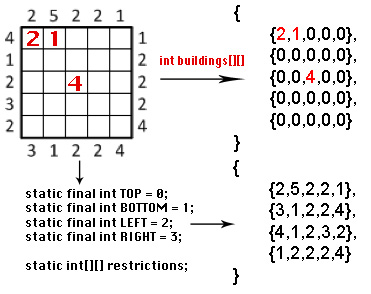
\includegraphics[scale=0.65]{./images/ModeladoSIA.jpg}
\label{modelado}
\end{center}
\end{figure}

\begin{center}
\par Figura 1: Modelado del problema
\end{center}


%\VerbatimInput{./code/calculoAb.m}




\end{document}